\documentclass[11pt]{article}
\pdfoutput=1

\usepackage[margin=1.15in]{geometry}
\usepackage{amsmath,amssymb}
\usepackage{booktabs}
\usepackage{graphicx}
\usepackage{microtype}
\usepackage{xcolor}
\usepackage[round]{natbib}
\usepackage[colorlinks=true, linkcolor=blue!50!black, citecolor=blue!50!black, urlcolor=blue!50!black]{hyperref}

\newcommand{\Rl}{R(\ell)}
\newcommand{\Gl}{G(\ell)}

\title{Does a Learned Market Simulator React?\\
\large Causal Injection Tests Against the Impact Kernel}
\author{Kareem Fareed\\
Stanford University\\
\texttt{kfareed@stanford.edu}}
\date{July 2026}

\begin{document}
\maketitle

\begin{abstract}
Backtests that replay recorded market data cannot account for market impact, because their recording never reacts to the strategy under test. 
Generative models of order flow promise to close this gap, but published evaluations of their reactivity compare stylized facts of free-running rollouts to real data, plot prices with and without an injected agent, or calibrate synthetic impact to aggregate impact laws; to our knowledge, none isolates the causal effect of a single exogenous order against a quantitative magnitude reference. We propose a causal evaluation protocol in which a single trade the model never generated is injected into real context, buy and sell arms are rolled out under common random numbers so that they differ by a single token, and the paired response is graded against a quantitative benchmark from market-microstructure theory, the impact kernel deconvolved from the order-sign autocorrelation under the propagator model. The benchmark is essential, because the average price move following a real trade is dominated by the correlated flow that accompanies it; on our data, the single-trade kernel is roughly an order of magnitude smaller than the raw response, so an evaluation against the wrong reference would misjudge a correct simulator severalfold. We apply the protocol to an 87M-parameter autoregressive transformer trained for 1.4B tokens on an 11.75B-token corpus of Binance perpetual-futures order flow, and report results from a test split used for neither training nor checkpoint selection. Across 2{,}048 paired injections per symbol, rolled out under positional common random numbers that share the sampling noise across arms position-by-position, the buy--sell contrast is positive with intervals clear of zero through at least lag 75 on every symbol at both injected order sizes on the frame clock, while the plateau comparison against each symbol's kernel discriminates sharply. SOL's response passes the pre-declared factor-two equivalence test against its kernel at both order sizes with kernel uncertainty propagated (ratio intervals $[0.68, 1.42]$ and $[0.94, 1.71]$, the former inside the stricter 1.5 margin as well), ETH's median-size response is positive but attenuated (point estimate $0.7\times$ its kernel, with neither equivalence nor the deficit resolved) and its large-order response inverts sign, and BTC, a negative control, responds significantly wrong-signed at both order sizes. None of this behavior is targeted by next-token training. A TWAP execution study quantifies the practical consequence. The reactive simulator charges 0.33--0.72 ticks per unit of size-dependent quote-response cost, a lower bound on execution cost that replay scores as zero. We argue that injection tests against the impact kernel should become a standard evaluation for learned market simulators.
\end{abstract}

\section{Introduction}

A typical backtest evaluates a candidate strategy by replaying recorded market data against it. The recording, however, never reacts. The strategy's fills are free, and the recorded price path is unaffected by any order the strategy submits. For strategies that trade meaningful size this is a severe deficiency, because the quantity a backtest most needs to estimate, the effect of the strategy's own trading on the price, is zero by construction.

Generative models of order flow offer a solution. A model trained to predict the next market event given history yields rollouts that constitute a synthetic market capable, in principle, of reacting. Once an injected order enters the model's context, everything generated afterwards is conditioned on it. A rapidly growing literature builds such simulators from GANs \citep{coletta2021,coletta2022}, autoregressive token models \citep{nagy2023}, masked-language-model encoders \citep{lobert2025}, diffusion models \citep{trades2025,difflob2026}, and order-level foundation models \citep{mars2025}.

Evaluation has not kept pace with model development. The standard tests are distributional, comparing spreads, volumes, inter-arrival times, and return moments between generated and real data \citep{cont2001,lobbench2025}. These are necessary conditions, but they cannot certify reactivity. A simulator can match every marginal and still respond incorrectly to an exogenous order, because distributional statistics are computed on rollouts in which the model only ever responds to its own flow. Where responsiveness is tested at all, the tests are coarse. A percentage-of-volume agent is activated and the resulting mid-price difference plotted \citep{coletta2022,trades2025}, or synthetic impact is calibrated to aggregate impact laws \citep{mars2025,noble2026}. None of these designs isolate the causal effect of a single exogenous order, and none compare the measured response to the quantity that microstructure theory predicts for one.

Market-microstructure theory provides the relevant quantitative reference. Because order signs have long memory \citep{lillofarmer2004}, the average price move following a buy is not the impact of that buy alone but the combined impact of the buy and the correlated buys that typically accompany it. The propagator model \citep{bouchaud2004,taranto2016} separates the two. The observed (dressed) response $\Rl$ is the single-trade impact kernel $\Gl$ convolved with the sign autocorrelation, so given measurements of $\Rl$ and the sign autocorrelation one can deconvolve for $\Gl$. An injected trade in a simulator is precisely an exogenous, uncorrelated trade, and its response should therefore be compared to the impact kernel rather than the dressed response. On our data the two differ by more than an order of magnitude, so an evaluation against the wrong reference would reject a correct simulator as several times too weak.

\paragraph{Contributions.} We propose and demonstrate a causal evaluation protocol for learned market simulators:

\begin{enumerate}
\item \textbf{Paired injection tests under positional common random numbers.} A single marketable order the model never generated is spliced into real context, and buy and sell arms are rolled out sharing their sampling noise position-by-position via Gumbel-argmax sampling, so that the paired difference $(R_{\mathrm{buy}}-R_{\mathrm{sell}})/2$ is a causal contrast between the two intervention signs and the pairing survives arbitrary divergence of the token histories, at an unchanged marginal sampling law. To pass, the response must have the correct sign, grow with order size, and match the correct magnitude.
\item \textbf{The impact kernel as a direct-effect reference.} We deconvolve the impact kernel from real trades under the propagator model. Because an exogenous trade may legitimately induce reaction, the primary structural prediction, derived from the propagator assumptions rather than guaranteed by them, is a bracketing, $G \le \hat{R}_{\mathrm{inj}} < R$, in which the injected response lies between the impact kernel and the dressed response. The bracketing holds on SOL, where the response is formally equivalent to the kernel at the pre-declared factor-two margin, and departures from it are themselves diagnostic. ETH's point estimate falls below the impact kernel, indicating under-reaction, although the deficit is not resolved once kernel uncertainty is propagated. We measure all three components separately and report closeness to $G$ as a secondary direct-effect calibration with pre-declared equivalence margins.
\item \textbf{A negative control by construction.} We run the identical protocol on a symbol selected as a negative control because independent distributional diagnostics indicate excess trend persistence. Its failure demonstrates that the protocol discriminates among causal behaviors rather than mechanically producing favorable outcomes.
\item \textbf{The replay gap} A TWAP execution strategy evaluated in replay, in the reactive simulator, and against a no-trade control identifies a quote-response cost of 0.33--0.72 ticks per unit.
\end{enumerate}

The demonstration vehicle is an 87M-parameter decoder-only transformer trained for 1.44B token presentations sampled from an 11.75B-token corpus of raw Binance perpetual-futures order flow (Section~\ref{sec:model}). To our knowledge, this is the first learned LOB simulator built and evaluated on cryptocurrency perpetual L2 data, published systems having trained on US or Chinese equity feeds. The methodology itself, however, is model-agnostic. Any generative order-flow model that can accept an injected event can be evaluated in the same way.

\section{Related work}
\label{sec:related}

\paragraph{Learned LOB simulators.} \citet{jain2024} survey the field, which spans hand-calibrated agent-based simulation, hybrid neural agents \citep{shi2023}, whose evaluation includes percentage-of-volume agent experiments contrasting responsive and non-responsive background flow, and fully learned generators. \citet{coletta2021,coletta2022} replace hand-calibrated multi-agent simulations \citep{abides2019} with a single conditional-GAN ``world agent'' trained on historical flow, evaluated with a stylized-fact battery and a percentage-of-volume (POV) agent injection measured as the average mid-price difference with and without the agent. \citet{nagy2023} introduce the first end-to-end autoregressive token-level generative model of LOB messages, with an LLM-style tokenizer and a state-space backbone; evaluation covers perplexity and marginal statistics, and the authors name realistic market impact as an open problem. LOBERT \citep{lobert2025} adapts a BERT-style foundation model to LOB messages, evaluated on prediction accuracy and marginal fidelity. On the diffusion side, TRADES \citep{trades2025} generates order flow conditioned on market state and demonstrates responsiveness qualitatively through a single POV-agent experiment. DiffLOB \citep{difflob2026} diagnoses the same passivity problem we target, observing that prior generative LOB models ``remain fundamentally passive'', but intervenes at the level of market regimes rather than individual orders. MarS \citep{mars2025} is the closest system-level work, an order-level autoregressive foundation model explicitly framed as language modeling for markets, demonstrated as an interactive simulator with a TWAP-agent experiment and a check that synthetic impact follows the square-root law. On the mechanistic side, \citet{noble2026} build an interactive simulator with an explicit impact-feedback term that reproduces concave in-execution impact and partial reversion; their feedback is specified and calibrated rather than learned, and validated against impact laws rather than by intervention on a learned generator.

\paragraph{Evaluation methodology.} LOB-Bench \citep{lobbench2025} is the emerging standard benchmark. It is explicitly distributional, measuring L1 and Wasserstein-1 divergences of conditional and unconditional statistics, plus discriminator scores, on US-equity LOBSTER data. Its impact metrics, including the response function $\Rl$, are computed on freely generated sequences matched to real ones, not under intervention, and its authors flag testing generated impact against impact laws as future work. Our protocol is complementary. Distributional batteries assess the simulator's unconditional behavior; injection tests assess its causal response to exogenous orders.

\begin{table}[t]
\centering
\small
\begin{tabular}{lll}
\toprule
Work & Generator & Responsiveness evaluation \\
\midrule
\citet{coletta2021,coletta2022} & conditional GAN & POV agent; mean mid-price difference \\
\citet{nagy2023} & AR token model (S5) & none (impact named as open problem) \\
\citet{trades2025} & diffusion & POV agent; qualitative \\
\citet{mars2025} & AR foundation model & TWAP demo; square-root-law check \\
\citet{difflob2026} & diffusion & regime-level counterfactuals \\
\citet{lobbench2025} & (benchmark) & $\Rl$ on free rollouts; no injection \\
\citet{noble2026} & mechanistic, impact feedback & calibration to impact laws \\
\midrule
This work & AR token model & paired single-trade injection, CRN, \\
& & dose scaling, kernel match, falsification \\
\bottomrule
\end{tabular}
\caption{How reactivity is evaluated across LOB simulators. To our knowledge, no prior work injects a single exogenous trade under paired common-random-number arms or compares the response to the deconvolved impact kernel.}
\label{tab:related}
\end{table}

\paragraph{Impact theory.} The propagator model \citep{bouchaud2004}, the long memory of order signs \citep{lillofarmer2004,lmf2005}, and their joint implications for response functions \citep{bouchaud2009,taranto2016,gatheral2010} provide the theory that underly our metrics. The square-root impact law \citep{toth2011} concerns metaorders executed against daily volume; Section~\ref{sec:replaygap} shows why it is the wrong benchmark for second-scale single-trade experiments, a distinction that also matters for interpreting simulator evaluations. \citet{naviglio2025} show that price models calibrated on public data typically get metaorder impact qualitatively wrong, which motivates evaluating learned simulators on exactly this axis.

\section{Data and representation}
\label{sec:data}

\paragraph{Corpus.} We use Binance USD-margined perpetual-futures incremental L2 depth and trade feeds from Tardis.dev, which makes the first day of every month freely available. The corpus comprises 198 training symbol-days of BTCUSDT, ETHUSDT and SOLUSDT spanning 2021 through mid-2026, plus one held-out day per symbol. A single day of BTC perpetual L2 alone contains 161M book events.

\paragraph{Feed structure.} Binance publishes depth \emph{diffs} on a fixed $\sim$26\,ms timer, with the 10th through 99th percentiles of inter-frame gaps all falling in 26--30\,ms, so book updates carry no event-time process of their own; event-time structure resides in the trades. A median frame carries 25 level changes and the 99th percentile carries over 200. The median book change occurs 403 ticks from the touch, and only 10--15\% occur within trading-relevant distance of it. The book is consistent only at frame boundaries, and is transiently crossed mid-frame roughly 10\% of the time.

\paragraph{Tokenization.} The representation is a single chronological stream. Every event opens with a log-bucketed $\Delta t$ token, followed by either a trade (side, price offset, size) or a frame (a list of near-touch level changes). Price offsets are expressed in ticks from the \emph{pre-event} same-side best, so generated events can be applied forward without self-reference; in-band offsets cover $-16$ to $+63$. Sizes use 32 log$_2$ buckets. All buckets are fixed a priori, so the tokenizer involves no fitting to data and introduces no leakage. The vocabulary is 384 tokens, an event averages $\sim$2.6 tokens, a market day is $\sim$65M tokens, and the available source corpus contains 11.75B tokens. The evaluated checkpoint was trained on 1.44B sampled token presentations from that corpus.

One representation detail matters particularly for backtesting. Price improvements beyond the in-band offset range are not rare. A cap at 16 ticks per frame per side would constrain us on 0.8\% of frames on a calm day and 3.2\% on a violent one, with the worst single frame improving the best bid by 1,272 ticks within 26\,ms and one 2021 frame moving 34,545 ticks. A two-digit base-32 \emph{jump escape} therefore encodes the improvement magnitude exactly up to 1,040 ticks; larger improvements are clamped. The escape reduces but does not eliminate this representation failure, which persists precisely where a backtesting simulator matters most: in the tails.

\section{Model and training}
\label{sec:model}

The model is a vanilla decoder-only transformer with 87M parameters, width 768, 12 layers, 12 heads, and a context of 2,048 tokens ($\sim$10--13\,s of market). Optimization uses the Muon optimizer (learning rate $2\times10^{-2}$, 500-step warmup) and continues for 26.5k steps ($\sim$1.74B token presentations, $\sim$20 per parameter). Validation loss selects the checkpoint at step 22{,}000, after $\sim$1.44B token presentations; this is the checkpoint evaluated throughout the paper. It reaches 1.375 nats/token on a strictly walk-forward validation set (the first half of 2026-07-01, one month after the final training day); the uniform baseline is $\ln 384 = 5.95$.

Decoding is grammar-constrained, masking any token that would be syntactically illegal at the current position. The constraint is rarely exercised, as the raw probability mass on illegal tokens is only 0.05--0.07\% per step, and rollouts are stable, with flat median and 90th-percentile spread over full two-minute rollouts on all three symbols.

\section{Distributional evaluation with a noise floor}
\label{sec:distributional}

Before asking whether the simulator reacts, we ask whether its free-running output is statistically realistic. Here and throughout, the evaluation is the same. The holdout day is split in half; the first (validation) half was used for checkpoint selection and for developing the protocol, including exploratory pilots. The second (test) half evaluates every statistic reported in this paper. We seed the model with 2,048 tokens of real test-split context, roll out, and compare the rollouts to test-split real data on a battery of statistics: spread and depth distributions (compared by Kolmogorov--Smirnov distance), event rates, economically impossible states (crossed books), return kurtosis and its aggregational decay, volatility clustering, and the variance signature plot.

\paragraph{A real-vs-real noise floor.} A KS distance of 0.1 is not interpretable in isolation, since even two disjoint windows of \emph{real} market data do not have identical distributions. We therefore compute each metric between two disjoint real windows and use this real-vs-real value as a noise floor. The model passes a metric when its generated-vs-real value lands near the real-vs-real value. Single-run KS values vary substantially across seed sets, so individual entries should be read as indicative rather than precise.

\paragraph{Stratification by symbol.} Pooled across symbols, the spread KS passes below the noise floor, but the pass is an artifact. Pooling allows cross-symbol composition to swamp within-symbol differences (SOL's spread distribution is nearly degenerate at one tick). Stratified by symbol, spread realism is mixed (Table~\ref{tab:scorecard}). Distributional evaluations of multi-asset generative models should therefore always be stratified.

\begin{table}[t]
\centering
\small
\begin{tabular}{lccc}
\toprule
generated (real) & BTC & ETH & SOL \\
\midrule
frames/s & 33.0 (35.9) & 38.7 (39.6) & 34.5 (32.9) \\
trades/s & 39.2 (60.7) & 154.4 (70.3) & 57.1 (31.2) \\
spread p50/p90/p99 (ticks) & 1/4/4 (1/2/5) & 1/1/18.6 (1/1/1) & 1/1/2 (1/3/3) \\
spread KS (noise floor) & 0.18 (0.10) & 0.015 (0.000) & 0.13 (0.29) \\
crossed frames per 1k (baseline) & 12.9 (10.7) & 13.9 (0.0) & 1.0 (0.0) \\
illegal mass per step & 0.05\% & 0.05\% & 0.06\% \\
\bottomrule
\end{tabular}
\caption{Stratified scorecard on the held-out test split (four 12k-token rollouts per symbol). Frame timing is close on all symbols, but generated trade rates run high on ETH and SOL (ETH more than doubles the real rate), ETH's spread tail occasionally blows out, and books run too deep on ETH and SOL (not shown). Free-running realism on the test half is visibly worse than a single-metric reading would suggest, which sharpens the question of whether causal responses survive.}
\label{tab:scorecard}
\end{table}

\paragraph{Emergent impact.} The first economic metric is the response function $\Rl = \mathbb{E}[\epsilon \cdot (m_{t+\ell}-m_t)]$, the average signed mid-price move following a trade. Although nothing in next-token training targets impact, the generated market reproduces the shape and short-lag magnitude of the real response on all three symbols (Figure~\ref{fig:impact}). The systematic failure appears at long lags. Real impact plateaus, whereas generated impact continues to climb, exceeding the real value by roughly 50\% at lag 100 on BTC and ETH.

\begin{figure}[t]
\centering
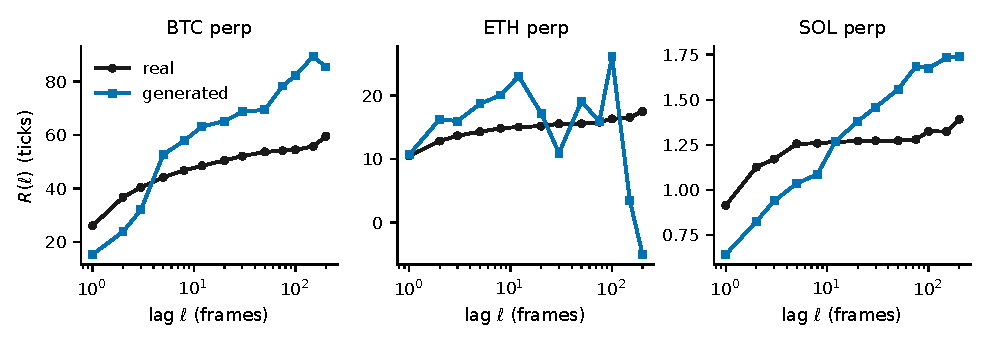
\includegraphics[width=\textwidth]{figures/impact.pdf}
\caption{Impact response function $\Rl$, real vs.\ generated, per symbol (lags in $\sim$26\,ms frames). Impact is emergent; nothing in training targets it. Short-lag magnitude and shape are close on all symbols; generated impact fails to plateau, most severely on BTC.}
\label{fig:impact}
\end{figure}

\paragraph{The mechanism is over-persistent order flow.} Real order signs exhibit slow power-law memory, $C(\ell)\sim\ell^{-\gamma}$ \citep{lillofarmer2004}. Fitting both real and generated flow (Figure~\ref{fig:signacf}) yields real $\gamma = 0.47/0.61/0.61$ on BTC/ETH/SOL against generated $0.22/0.19/0.50$. Generated flow is too persistent on every symbol, with the memory gap smallest on SOL (0.10) and largest on ETH (0.42). The ranking of the gap loosely matches the ranking of the impact overshoot on this data. The two diagnostics share a single candidate mechanism. The model over-continues flow, and in a market with transient impact, over-persistent flow prevents the response from plateauing.

\begin{figure}[t]
\centering
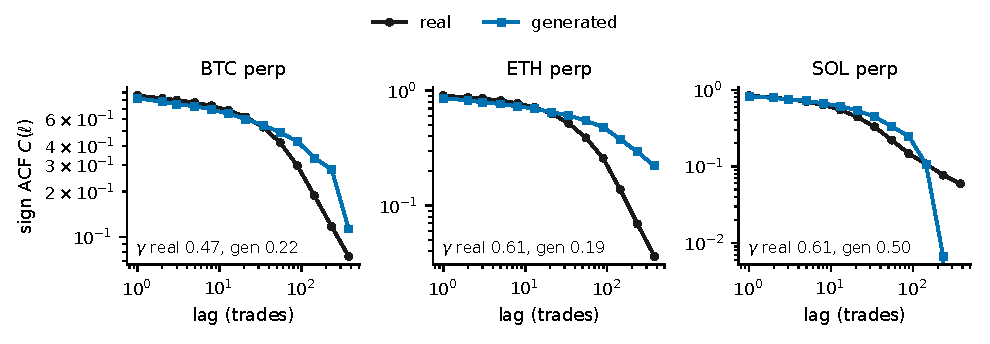
\includegraphics[width=\textwidth]{figures/signacf.pdf}
\caption{Order-sign autocorrelation, log--log. Generated flow (blue) is more persistent than real (black) on every symbol; the $\gamma$ gap is largest on ETH (0.42) and smallest on SOL (0.10).}
\label{fig:signacf}
\end{figure}

These distributional results establish the setting for what follows. Free-running realism on the test split is imperfect and strongly symbol-dependent, with ETH degrading the most. Whether causal responses degrade in the same way is precisely the question the injection protocol answers directly, and, as Section~\ref{sec:results} shows, the answer is not what the distributional picture suggests.

\section{Injection methodology}
\label{sec:method}

The distributional battery leaves one question unanswered. Does the model treat an exogenously submitted order as information? The model was trained to predict the next token of real flow; nothing guarantees that it treats an exogenous trade as anything but noise.

\paragraph{Design.} We take 2{,}048 windows of real test-split context per symbol (1,532 tokens each, cut at event boundaries, spanning each symbol's test region). For each window we run five arms sharing the identical context, a marketable buy at the touch and a marketable sell at the touch, each at two doses, the median trade size ($1\times$) and three size buckets larger ($\approx 8\times$), plus a no-injection control. The injected trade is spliced in as four tokens ($\Delta t$, side, offset~0, size). Each arm then generates 2,500 new tokens, so the buy and sell rollouts differ by exactly one token of input, and the paired statistic
\[
\hat{R}_{\mathrm{inj}}(\ell) \;=\; \tfrac{1}{2}\,\big(R_{\mathrm{buy}}(\ell) - R_{\mathrm{sell}}(\ell)\big)
\]
is a causal contrast between the two intervention signs; it equals the effect of a buy relative to no order only under buy/sell antisymmetry, which we test rather than assume (Section~\ref{sec:results}). The control arm measures residual drift. A bookkeeping check verifies that each spliced trade is parsed as intended and that the rollout contains enough post-injection trades to reach the plateau window; the pairs entering the plateau statistic number 1{,}991 and 1{,}997 of 2{,}048 at the two doses on SOL, 1{,}998 and 1{,}997 on ETH, and 2{,}021 and 2{,}017 on BTC. Confidence intervals throughout are 95\% percentile bootstraps over seeds (2{,}000 resamples) unless noted; equivalence tests use 90\% intervals as required by the two-one-sided-test construction.

\paragraph{Positional common random numbers.} Pairing the arms is what gives the contrast its power, and ordinary common random numbers pair imperfectly. With a shared-seed sampler, the arms consume the same underlying random draws, but the coupling between their emitted tokens weakens once their histories, and hence their conditional distributions, diverge. We instead make the coupling explicit and position-stable by sampling each token with Gumbel-argmax. For window $w$, a per-window noise stream advanced once per output position yields a vocabulary-sized Gumbel vector $g_{w,t}$ that is a deterministic function of $(w,t)$ alone, and the emitted token is $\arg\max_v (z_v/T + g_{w,t,v})$ over the grammar-legal logits $z$. Per position this reproduces exactly the masked softmax sampling law, so the marginal distribution of each rollout is unchanged, but because the noise is indexed by position rather than by sampling history, all five arms of a window share their entire noise realization no matter how far their token streams diverge. On our data this coupling reduces the variance of the paired plateau statistic by roughly a factor of two relative to ordinary shared-seed sampling, at no cost in generation; on SOL at the median dose the per-seed standard deviation of the paired statistic is $0.32$ ticks.

\paragraph{Criteria fixed in advance.} Three tests were fixed before results. \emph{Sign}: the paired response must be positive with confidence intervals clear of zero. \emph{Dose}: the $8\times$ injection must produce a larger response than $1\times$. \emph{Magnitude}: the response must be quantitatively right, which requires knowing what ``right'' is. The magnitude test is scored in the kernel's plateau window (trade lags 16--24, where the real $G$ has flattened) as the per-seed mean over those lags, bootstrapped across seeds, and formalized as a two-one-sided equivalence test with margins declared before any test-split data was analyzed, a primary margin of a factor of two around the kernel (``same scale'') and a secondary margin of 1.5.

\paragraph{The magnitude yardstick.} The natural candidate is the measured response to real trades, $R(\ell)$, but it is the wrong target. Real order flow is autocorrelated ($C(1)=0.840$ on SOL). A real buy is accompanied by the correlated buys that typically follow it, so $R(\ell)$ reflects the aggregate effect of that correlated flow. An injected trade carries no such flow; it is exogenous by construction. Under the propagator model \citep{bouchaud2004,taranto2016}, the dressed response is the impact kernel convolved with the sign autocorrelation,
\[
R(\ell) \;=\; G(\ell) \;+\; \sum_{0 < |k|} G(\ell - k)\, C(k) \quad\text{(schematically)},
\]
so given measurements of $R$ and $C$ on real data one can solve the linear system backwards for the impact kernel $G$. We do this per symbol, on 336k--504k real test-split trades over 64 trade lags; Appendix~\ref{app:deconv} gives the exact estimators, the discretized system, its failure modes, and identification robustness. The deconvolved kernels plateau over trade lags 16--24 at $+0.032$ ticks on SOL, $+0.175$ on ETH, and $+0.423$ on BTC, in each case more than an order of magnitude below the dressed response at the same lags. Identification quality differs sharply across symbols. A truncation-horizon sweep moves the SOL kernel by under 20\% ($0.038$ to $0.032$ across $L=32$--$64$; segment bootstrap $[0.027, 0.036]$), the ETH kernel by 60\% at the shortest horizon ($0.263$ at $L=32$, stabilizing at $0.164$--$0.187$), and the BTC kernel by a factor of $2.2$ ($1.13$ to $0.51$), so the BTC kernel is at best loosely identified. One caution governs the interpretation. Deconvolution removes correlated future flow regardless of whether that flow is confounding (a latent metaorder that the trade merely signals) or a genuine reaction that the trade causes, so $G$ is a \emph{direct-effect} reference rather than the unique causal truth. The total response to an exogenous trade may legitimately exceed $G$ through induced reaction, while the fully dressed $R$ prices the entire historical correlated crowd. Under the propagator assumptions, with a nonnegative kernel and induced flow no stronger than the historical correlated flow, the response is predicted to fall between the two; we present this bracketing as the primary structural diagnostic, under those stated assumptions, rather than as a bound that cannot be violated:
\[
G_{\mathrm{real}} \;\le\; \hat{R}_{\mathrm{inj}} \;<\; R_{\mathrm{real}},
\]
with closeness to $G$ serving as a secondary direct-effect calibration. Both the ordering and the induced follow-on flow are directly observable in the rollouts.

\section{Injection results}
\label{sec:results}

\begin{figure}[t]
\centering
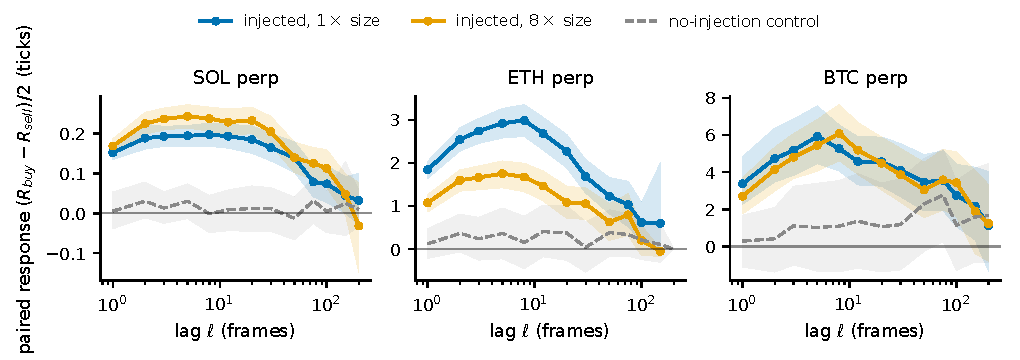
\includegraphics[width=\textwidth]{figures/injection.pdf}
\caption{Paired injection response on the held-out test split, with bootstrap 95\% bands, 2{,}048 seeds per symbol; note the differing y-scales. The frame-clock response is positive with intervals clear of zero through at least lag 75 on every symbol at both doses, so at these lags the sign criterion does not discriminate; the trade-clock plateau comparison of Figure~\ref{fig:plateau} does. The no-injection controls are consistent with zero at every lag on SOL and ETH; BTC's control drifts positive at lag 75 (pointwise).}
\label{fig:injection}
\end{figure}

\paragraph{Sign.} On the frame clock the paired buy-minus-sell response is positive with bootstrap intervals clear of zero through lag 100 on SOL at both doses, through lag 100 at $1\times$ and lag 75 at $8\times$ on ETH, and through lag 150 at $1\times$ and lag 100 at $8\times$ on BTC (Figure~\ref{fig:injection}); at short and intermediate lags the sign criterion therefore does not discriminate among the symbols. The control arms drift by amounts consistent with zero at every measured lag on SOL and ETH; BTC's control is positive at lag 75 ($2.8$ $[0.3, 5.3]$, pointwise), a further sign of its instability. Injection leaves the model's syntax undisturbed (illegal probability mass is unchanged). The spread and crossed-frame marginals of injected rollouts remain of the same order as the control arm's, although BTC exhibits some injection-conditioned deterioration in the upper tail (90th-percentile spread 2.6 ticks in control against 2.8--3.2 across injected arms; medians 1.9 against 1.9--2.2). The discrimination appears at the trade-clock plateau, where responses are compared against each symbol's kernel.

\paragraph{Dose.} An $8\times$ order should not be expected to produce an $8\times$ response. The size-conditioned response of real trades is nearly flat (Section~\ref{sec:replaygap}), so the causal response should grow far more slowly than proportionally. On SOL the paired dose difference is $+0.008$ $[-0.005, +0.019]$, consistent with both zero and a shallow dependence; the pre-declared dose criterion, a strictly larger response at $8\times$, is therefore not established even where everything else passes. On ETH the large dose \emph{fails}. The paired dose difference is $-0.173$ $[-0.254, -0.092]$, significantly negative, and the $8\times$ response itself is wrong-signed ($-0.059$, with a 95\% interval $[-0.120, -0.0003]$ that only marginally excludes zero, but a temporal-block interval $[-0.108, -0.016]$ that excludes it clearly; Appendix~\ref{app:robust}). The model under-responds to large injected trades on ETH; a plausible mechanism is that the injected size bucket is rare in ETH's flow, leaving the large injection partially out of distribution. This failure is invisible to distributional evaluation and is precisely the kind of defect the protocol exists to catch.

\paragraph{Magnitude.} Figures~\ref{fig:kernel} and~\ref{fig:plateau} present the central result. On SOL the plateau response is $+0.033$ $[+0.019, +0.046]$ at $1\times$ and $+0.042$ $[+0.029, +0.054]$ at $8\times$ against a kernel of $+0.032$, point estimates at $1.0$ and $1.3\times$ the kernel, inside the predicted bracket $[G, R)$, and stable under temporal-block resampling (Appendix~\ref{app:robust}). Formal equivalence at the pre-declared factor-two margin is established at both doses. With kernel uncertainty propagated by a ratio bootstrap (Appendix~\ref{app:robust}), the SOL ratio intervals are $[0.68, 1.42]$ at $1\times$ and $[0.94, 1.71]$ at $8\times$, both inside $[1/2, 2]$, and the $1\times$ interval also passes the stricter secondary margin of 1.5. On ETH the median-size plateau response is positive ($+0.123$ $[+0.044, +0.196]$) but attenuated. The point estimate is $0.71\times$ its kernel of $+0.175$, and the 90\% ratio interval $[0.33, 1.06]$ establishes neither equivalence at either margin nor a resolved deficit, so the bracketing fails from below at the point-estimate level while the sample leaves the under-reaction short of significance. Nothing in training targets these quantities; they emerge from next-token prediction on raw flow. Under the three pre-specified criteria, SOL passes sign and magnitude while its dose criterion remains unestablished (the difference is positive but consistent with zero, as the near-flat empirical size dependence predicts); ETH and BTC fail. The supported claim is formal factor-two equivalence on SOL and point-estimate attenuation, without a statistically resolved deficit, on ETH.

\begin{figure}[t]
\centering
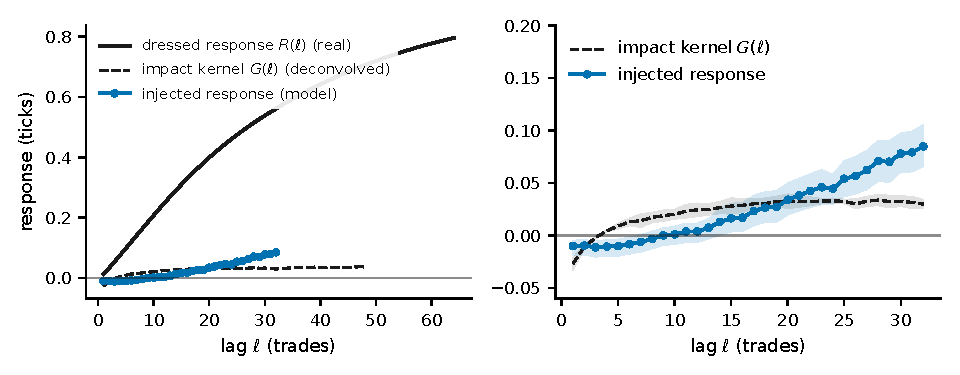
\includegraphics[width=\textwidth]{figures/kernel.pdf}
\caption{Dressed response, impact kernel, and injected response (SOL, trade-clock lags, test split). Left: the dressed response $R(\ell)$ to real trades dwarfs both the deconvolved impact kernel $G(\ell)$ and the model's injected response; comparing injections to $R$ would therefore misjudge the simulator by an order of magnitude. Right: zoomed. The injected response (blue, 95\% bootstrap band) runs at the kernel's scale, sitting somewhat above it through the plateau.}
\label{fig:kernel}
\end{figure}

\begin{figure}[t]
\centering
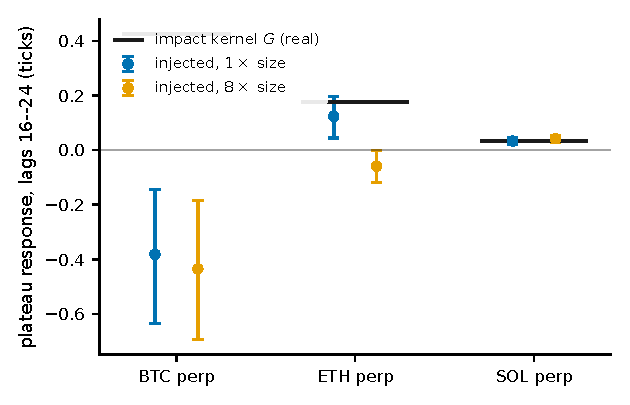
\includegraphics[width=0.62\textwidth]{figures/plateau.pdf}
\caption{The magnitude test on the held-out test split (2{,}048 seeds). Per-seed plateau-window (trade lags 16--24) injected response with 95\% bootstrap intervals, against the impact kernel deconvolved from each symbol's real trades (black bars). SOL's response passes factor-two equivalence to its kernel at both doses; ETH's median-size response falls below its kernel at the point estimate and its large-dose response inverts sign; BTC's response is significantly wrong-signed at both doses. BTC's kernel itself is only loosely identified (Appendix~\ref{app:deconv}).}
\label{fig:plateau}
\end{figure}

\paragraph{Induced flow, and what the estimand is.} The model interprets a single exogenous trade as part of a metaorder. The paired buy--sell contrast in the sign of the next generated trade is $+0.43$ on SOL, $+0.57$ on ETH, and $+0.42$ on BTC, decaying over tens of trades, consistent with the model's slightly elevated endogenous sign autocorrelation. This induced herding is why the SOL response sits at or above the impact kernel within the bracket. Two caveats delimit the estimand. First, the paired statistic is a causal contrast between buy and sell interventions rather than a buy-versus-no-order effect; decomposed against the control arm, all four SOL single-arm effects are individually significant with the correct signs (at $1\times$, buy $+0.030$ $[+0.004, +0.054]$ and sell $-0.035$ $[-0.064, -0.009]$), whereas ETH's decomposition is asymmetric. At $1\times$ the sell arm carries the effect ($-0.177$ $[-0.307, -0.033]$; buy $+0.070$, not resolved) and at $8\times$ the buy arm is itself significantly wrong-signed ($-0.124$ $[-0.236, -0.018]$). Second, the buy/sell antisymmetry that would equate the contrast with twice the single-arm effect is consistent with zero in all six symbol-dose cells.

\paragraph{BTC as a negative control.} A passing result is informative only if the test is capable of failing, so we include BTC as a selected negative control. Its generated flow independently exhibits severe sign-memory excess and non-plateauing impact on the distributional battery (Section~\ref{sec:distributional}), so the distributional diagnostics predict failure before any injection is run. The test fails at both doses. The plateau response is significantly wrong-signed at $1\times$ ($-0.38$, 95\% CI $[-0.64, -0.15]$) and at $8\times$ ($-0.43$, 95\% CI $[-0.69, -0.18]$), both retained under temporal-block resampling; an injected buy \emph{lowers} the mid at plateau horizons while the frame-clock response reads positive, so the response is internally contradictory across clocks. The deterioration is driven by the buy arms (at $8\times$, buy-minus-control is $-0.94$ $[-1.84, -0.13]$), and BTC's own real kernel is the least identified of the three, moving by a factor of $2$ under the truncation sweep. A simulator whose causal response is wrong-signed where it is measurable and unmeasurable elsewhere cannot support agent evaluation. The instrument discriminates; that is the purpose of the negative-control arm.

\paragraph{Distributional health does not determine causal quality.} A natural hypothesis is that the sign-memory gap orders injection outcomes. The healthier a simulator's free-running flow, the better its causal responses. On this data the association is directionally present but coarse. SOL, with the smallest gap ($0.10$), is the only symbol whose response certifies equivalence to its kernel, while ETH ($0.42$) and BTC ($0.25$) both fail, but in qualitatively different ways that the gap does not predict. ETH responds at $0.7\times$ its kernel at median size and inverts at large dose while keeping the correct frame-clock sign, whereas BTC's plateau is wrong-signed beneath a healthy-looking frame-clock response. Free-running diagnostics alone would reveal neither failure mode. Measuring causal behavior directly remains necessary, which is what the protocol provides.

\section{Quantifying the replay gap}
\label{sec:replaygap}

The injection tests certify the mechanism. The remaining economic question is how much the reactivity matters for the backtests the simulator exists to serve.

\paragraph{Design.} The strategy is a TWAP taker that must buy a fixed quantity on SOL as $K=8$ marketable child orders at the touch, spaced 250 generated tokens apart. We evaluate it in three ways over 256 seeds: under \emph{naive replay}, where fills occur at recorded prices and the market cannot react; under the \emph{reactive} simulator, where each child order is injected and generation continues from it; and against a \emph{no-trade control} in the same generated market under common random numbers, which isolates background drift. Execution cost is implementation shortfall (mean child fill price minus arrival mid, in ticks per unit), and the strategy's self-caused impact is the reactive shortfall minus the control shortfall. Child size is swept over four doses spanning $\tfrac{1}{8}\times$ to $64\times$ the median trade size, a $512\times$ range. One mechanical limitation defines what is measured. Injected child orders enter the simulator as trade prints and are filled at the prevailing best ask regardless of size, without consuming book depth. The measured cost is therefore the generated market's \emph{quote response} to the strategy's trade prints, a component of execution cost that excludes walking the book, and the resulting figures are lower bounds on total impact cost.

\begin{figure}[t]
\centering
\begin{minipage}[t]{0.48\textwidth}
\centering
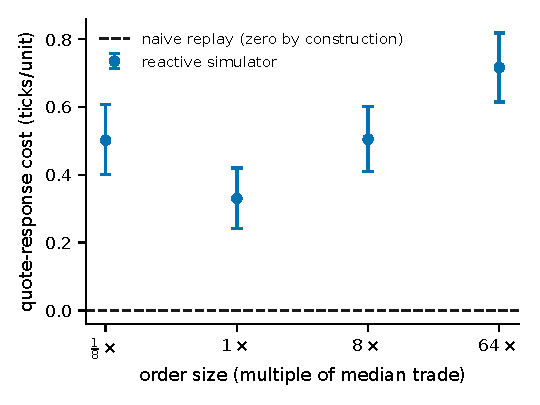
\includegraphics[width=\textwidth]{figures/pnlgap.pdf}
\end{minipage}\hfill
\begin{minipage}[t]{0.48\textwidth}
\centering
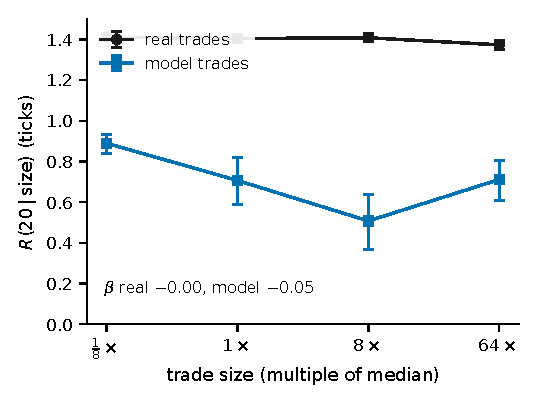
\includegraphics[width=\textwidth]{figures/size.pdf}
\end{minipage}
\caption{Left: the replay gap on the test split. Naive replay charges zero impact by construction; the reactive simulator charges a quote-response cost of 0.33--0.72 ticks per unit (bootstrap 95\% CIs, 256 seeds), largest at the largest dose and non-monotone at small doses. Right: validating the flat size dependence against reality. The size-conditioned response to \emph{real} SOL trades is flat across a 512$\times$ size range (exponent $-0.004$); the model's own trades reproduce the flatness at a level roughly half the real one.}
\label{fig:pnl}
\end{figure}

\paragraph{Replay understates a real cost.} Naive replay's impact is identically zero. The reactive simulator charges $+0.33$ to $+0.72$ ticks per unit across the dose range, every interval clear of zero (Figure~\ref{fig:pnl}, left). The cost is largest at the largest dose ($+0.72$ $[+0.62, +0.82]$ at $64\times$) but is not monotone at small doses ($+0.50$ at $\tfrac{1}{8}\times$ against $+0.33$ at $1\times$), so we do not fit a parametric size law. The robust statement is simpler. A replay backtest scores this entire cost, roughly half a tick per unit, as zero.

\paragraph{Flat size dependence reflects the data, not a model defect.} The square-root impact law is among the most robust facts in microstructure \citep{toth2011}, so nearly flat size dependence might suggest a model failure. It does not. The law describes metaorders executed against daily volume, whereas this experiment probes single marketable orders over seconds, a different quantity at a different timescale \citep{bouchaud2009}. Measured identically on the real test split, the size-conditioned response is \emph{flat} across a 512$\times$ size range (exponent $-0.004$; Figure~\ref{fig:pnl}, right). The model reproduces this flatness (exponent $-0.05$) at a level roughly half the real one, so if anything it understates large-order impact, an error in the conservative direction. The conditional flatness partly reflects selection, since large real trades are placed when the book can absorb them; a causal size dependence, if present, need not appear in this conditional measurement.

\section{Limitations}
\label{sec:limits}

The scope of this study is one venue, one asset class, and one calendar day, Binance perpetual futures across three symbols, with the test split being the second half of the same day whose first half served for validation, so cross-day and cross-venue generalization are untested. The exchange's 26\,ms frame cadence is the feed's ceiling and therefore the model's; only near-touch book state is modeled, sizes are log-bucketed, and trades see a book up to 26\,ms stale. The magnitude evidence certifies factor-two equivalence on SOL only, and the stricter 1.5 margin only at the median dose; the certification also inherits every propagator-model assumption baked into the kernel. The reported intervals quantify within-run sampling uncertainty; variability across independent evaluation runs with different generation seeds can exceed them, ETH's point estimates being the most sensitive. The impact-size curve rests on four coarse dose points and a single TWAP schedule. Injected orders enter the simulator as trade prints rather than mechanically executed market orders. Fills occur at the prevailing best quote regardless of size and book depth is not consumed, so all execution-cost figures are quote-response lower bounds; a matching engine with depth consumption is left to future work. The kernel deconvolution is an exact linear solve whose residual carries no statistical information; we report per-segment variability as the error bar, and the kernel is unstable at the first few lags (near-collinearity with $C(1)$ and bid--ask bounce) and at the horizon edge. Finally, there is a fundamental epistemic limitation. Validating the causal magnitude against real data is impossible in principle, because one cannot inject a trade into a recording. The deconvolved kernel is a model-based estimate of the causal quantity, not an experimental one. That impossibility is also the reason learned simulators are worth building, since they provide the intervention that data cannot, and it is precisely why their causal behavior must be tested rather than assumed.

\section{Conclusion}

A model trained only to predict the next token of order flow reacts causally to trades it never generated. On a held-out test split, the paired buy--sell contrast is positive for at least seventy-five frames on every symbol and dose, and on SOL the plateau response is formally equivalent to the impact kernel deconvolved from real trades at the pre-declared factor-two margin at both doses, inside the predicted bracket between the kernel and the dressed response; only the dose-monotonicity criterion remains unestablished there. The protocol's value is diagnostic as much as confirmatory. It exposes ETH's attenuated median-size response and large-dose sign inversion and the negative control's wrong-signed plateau at both doses, failures invisible to distributional evaluation. The practical consequence is also measurable. On our data, replay backtests omit a self-caused quote-response cost of 0.33--0.72 ticks per unit, itself a lower bound on the full execution cost.

The broader argument is methodological. The field is converging on generative order-flow models as reactive backtesters but grades them almost entirely on distributional realism, which cannot certify the one property that reactive backtesting requires, a correct causal response to exogenous orders. Paired injection tests against the impact kernel are inexpensive, model-agnostic, and falsifiable, and we suggest that they join stylized facts and distributional benchmarks as standard evaluation for any simulator intended to support interactive strategy evaluation. Code and evaluation outputs to reproduce all experiments will be made available at \url{https://github.com/KookiesNKareem/orderflow-lm}.

\bibliographystyle{plainnat}
\bibliography{refs}

\appendix

\section{Details of the kernel deconvolution}
\label{app:deconv}

This appendix specifies the estimator behind the yardstick in Sections~\ref{sec:method}--\ref{sec:results}, covering what is measured, the linear system that is solved, why its residual carries no statistical information, how uncertainty is estimated, and the regimes in which the estimate is known to be unreliable.

\subsection{Estimands and estimators}

All quantities in this appendix are computed on the trade clock (lags count trades rather than frames), because the propagator model is formulated at the level of trades. Let $\epsilon_i \in \{+1,-1\}$ be the sign of the $i$-th trade and $m_i$ the mid-price (in ticks; the mid has half-tick resolution) prevailing at that trade. The two measured objects are the dressed response and the sign autocorrelation,
\[
\hat{R}(\ell) = \frac{1}{N_\ell}\sum_i \epsilon_i\,(m_{i+\ell}-m_i),
\qquad
\hat{C}(\ell) = \frac{1}{N_\ell}\sum_i \epsilon_i\,\epsilon_{i+\ell},
\]
estimated on four disjoint segments of 2M tokens each, drawn evenly from the largest contiguous region of the test split for each symbol and replayed to book states (335{,}658 trades on SOL, 368{,}533 on ETH, 503{,}508 on BTC; sums pooled across segments). $\hat{R}$ and $\hat{C}$ are estimated for $\ell = 1,\dots,L$ with $L=64$, the range the discretized system below requires. On SOL $\hat{C}(1)=0.840$, $\hat{C}(8)=0.636$, $\hat{C}(32)=0.344$, $\hat{C}(64)=0.195$, $\hat{C}(127)=0.117$, the long memory of Section~\ref{sec:distributional}, now on the trade clock.

\subsection{The linear system}

The propagator model \citep{bouchaud2004} writes the mid as a linear superposition of transient single-trade impacts,
\[
m_i \;=\; \sum_{j<i} G(i-j)\,\epsilon_j \;+\; \eta_i,
\]
with $\eta$ noise uncorrelated with signs. Substituting into the definition of $R(\ell)$ and using $\mathbb{E}[\epsilon_i\epsilon_j]=C(|i-j|)$, $C(0)=1$:
\begin{align*}
R(\ell) &= \mathbb{E}\big[\epsilon_i\,(m_{i+\ell}-m_i)\big]
= \sum_{m=1}^{\ell} G(m)\,C(\ell-m) \;+\; \sum_{k\ge 1}\big[G(k+\ell)-G(k)\big]\,C(k)\\
&= \sum_{m\ge 1}\big[C(|m-\ell|)-C(m)\big]\,G(m).
\end{align*}
The first sum is the direct impact of the trades between $i$ and $i+\ell$, weighted by their correlation with trade $i$; the second captures the decay of impacts already in progress. Truncating at $m \le L$ gives a square system $A\,G = R$ with
\[
A_{\ell m} \;=\; C(|m-\ell|) - C(m), \qquad \ell, m = 1,\dots,L,
\]
which uses $C$ out to lag $L$ and is solved by least squares.

\subsection{Truncation}

Truncation drops the terms $[C(|m-\ell|)-C(m)]\,G(m)$ for $m > L$, and at $L=64$ the sign ACF has \emph{not} decayed ($C(64)=0.195$ on SOL), so the truncation requires justification. Each dropped weight is a difference of the slowly varying function $C$ evaluated at points $\ell$ apart. For $\ell \ll m$ it is small precisely because $C$ decays as a slow power law, and it grows as $\ell$ approaches $L$. The approximation is therefore accurate at the plateau lags we quote (16--24) and worst at the horizon edge, which is exactly where the recovered kernel visibly destabilizes (the upturn beyond lag $\sim$48 in Figure~\ref{fig:kernel}, left, is excluded from the plot and from all quoted numbers).

\subsection{Residuals and uncertainty}

$A$ is square and full rank, so the least-squares solution interpolates $\hat{R}$ essentially exactly (fit RMS $\approx 10^{-15}$ ticks). The residual is numerical, not statistical, and carries no information about estimation error. Uncertainty is instead estimated by repetition. $\hat{R}$ and $\hat{C}$ are re-estimated on each of the four segments separately, each segment is deconvolved on its own, and the cross-segment standard deviation of $G$ is reported as the band in Figure~\ref{fig:kernel} ($\pm 0.003$--$0.007$ ticks at the plateau on SOL, against a plateau level of $\approx 0.032$).

\subsection{Known failure modes}

The estimate has three known artifacts. (i) \emph{Short lags.} $G(1..3)$ comes out slightly negative on SOL ($-0.027$, $-0.011$, $-0.002$). There are two causes. Bid--ask bounce violates the pure propagator specification at lag 1, and with $C(1)=0.840$ adjacent columns of $A$ are nearly collinear, so the shortest lags are the least identified. Plateau values are unaffected. (ii) \emph{Horizon edge.} As above, lags near $L$ absorb the truncation error. (iii) \emph{Linearity.} The propagator assumes additive, size-independent impact. We deconvolve at the aggregate level and compare against injections at the median trade size; the near-flat conditional size dependence of the real response (Figure~\ref{fig:pnl}, right) makes this assumption benign in the regime where the comparison is made.

\subsection{The injected response on the same clock}

For a like-for-like comparison the pilot's injected responses are recomputed on the trade clock. In each injected stream the exogenous trade is, by construction, the $(n{+}1)$-th trade, where $n$ is the number of trades in the shared seed context; a bookkeeping check verifies that this trade's sign matches its arm and that the rollout reaches the plateau window, discarding the pair otherwise (valid pairs at the two doses number 1{,}991 and 1{,}997 of 2{,}048 on SOL, 1{,}998 and 1{,}997 on ETH, 2{,}021 and 2{,}017 on BTC). The per-seed response at trade lag $\ell$ is $m_{\tau(n+1+\ell)} - m_{\tau(n+1)}$, where $\tau(\cdot)$ indexes trades; arms are paired per seed as in Section~\ref{sec:method}, with percentile-bootstrap intervals over the 2{,}048 seeds (2{,}000 resamples). The plateau statistic of Section~\ref{sec:results} is the per-seed mean of this response over trade lags 16--24, bootstrapped across seeds. The induced-flow curve is the paired net sign of the $\ell$-th generated trade after the injection, computed from the same streams. The diagnostic ``endogenous kernel'' for the negative-control arm (Section~\ref{sec:results}) runs the identical $\hat{R},\hat{C} \to G$ pipeline on the control-arm rollouts' post-context trades ($L=24$; 102{,}839 trades on SOL, 191{,}097 on BTC).

\subsection{Identification robustness}
\label{app:robust}

Because the square system's residual carries no information, the kernel's stability is established by sweeping the truncation horizon $L$ over $\{32, 40, 48, 64\}$ and a Tikhonov ridge over $\lambda \in \{0, 10^{-3}, 10^{-2}, 10^{-1}\}$ (scaled by the mean diagonal of $A^{\!\top}\!A$), and by a segment bootstrap (twelve 1M-token segments resampled with replacement, 2{,}000 draws, re-pooling $\hat R$ and $\hat C$ jointly before deconvolving). Plateau values, in ticks:

\begin{center}
\small
\begin{tabular}{lcccc c}
\toprule
 & $L=32$ & $L=40$ & $L=48$ & $L=64$ & bootstrap 95\% CI ($L=64$) \\
\midrule
SOL & 0.038 & 0.034 & 0.032 & 0.032 & $[0.027, 0.036]$ \\
ETH & 0.263 & 0.176 & 0.164 & 0.187 & $[0.164, 0.212]$ \\
BTC & 1.129 & 0.673 & 0.562 & 0.509 & $[0.404, 0.621]$ \\
\bottomrule
\end{tabular}
\end{center}

The ridge sweep shrinks each kernel modestly and monotonically (SOL to $0.023$, ETH to $0.120$, BTC to $0.336$ at $\lambda = 10^{-1}$). SOL's kernel is stable to within 20\% across all specifications; ETH's stabilizes for $L \ge 40$; BTC's moves by a factor of $2.2$ and should be treated as loosely identified, which is reflected in the qualitative treatment of BTC in Section~\ref{sec:results}. The segment bootstrap resamples twelve evenly spaced segments of $10^6$ tokens each. The equivalence tests of Section~\ref{sec:results} are run with kernel uncertainty propagated by a ratio bootstrap (response draws over kernel draws, with the kernel draws recentred on the propagator-plateau kernel that serves as the reference throughout, so that numerator and denominator agree in expectation; equivalence requires the 90\% ratio interval inside $[1/2, 2]$). The SOL ratio intervals are $[0.68, 1.42]$ and $[0.94, 1.71]$ (equivalence established at both doses, and at the 1.5 margin for the former), and the ETH $1\times$ ratio interval $[0.33, 1.06]$ neither establishes equivalence nor excludes one, and its upper end is sensitive to the choice of kernel estimator (the segment-bootstrap and propagator-plateau estimators differ by 7\% on ETH), so the under-reaction is reported at the point-estimate level only. A temporal-block bootstrap over contiguous window blocks (sizes 16 and 64) accompanies every plateau interval. Blocked intervals move only modestly (SOL $8\times$, $[+0.030, +0.054]$ at block size 64) and are cited in Section~\ref{sec:results} wherever a significance statement is sensitive to them. Response and kernel are estimated from the same trading day, and residual same-day dependence between them is not modeled.

\end{document}
